\input{../article_base.tex}
\title{פתרון מטלה 07 --- משוואות דיפרנציאליות, 80320}
% chktex-file 9
% chktex-file 17

\usepackage{pgfplots, tikz, pgffor}
\usetikzlibrary{math}
\pgfplotsset{compat=1.18}

\begin{document}
\maketitle
\maketitleprint[blue]{}

\question{}
נגדיר את מערכת המשוואות,
\[
	\begin{pmatrix}
		x' \\
		y'
	\end{pmatrix}
	= \begin{pmatrix}
		y \\
		-y - \sin x
	\end{pmatrix}
\]

\subquestion{}
נמצא את נקודות שיווי המשקל של המערכת.
\begin{solution}
	נסמן $F : \RR^2 \to \RR^2$ המוגדרת על־ידי,
	\[
		F(x, y) = (y, -y - \sin x)
	\]
	ולכן מערכת המשוואות $(x, y)'(t) = F((x, y)(t))$ היא בדיוק המערכת שהגדרנו, ובהתאם $F$ מגדירה את הזרימה שלה.
	נקודה היא נקודת שיווי משקל אם $F(p) = 0$ ולכן נחשב נקודות אלה,
	\[
		F(x, y) = 0
		\iff \begin{cases}
			y = 0 \\
			-y - \sin x = 0
		\end{cases}
		\iff y = 0, \sin x = 0
	\]
	ולכן נקודות שיווי המשקל הן בדיוק $\pi \ZZ \times \{ 0 \}$.
\end{solution}

\subquestion{}
נקבע את היציבות של נקודות שיווי המשקל שמצאנו.
\begin{solution}
	\[
		DF|_{(x, y)}
		= \begin{pmatrix}
			0 & 1 \\
			- \cos x & -1
		\end{pmatrix}
	\]
	בפרט עבור $x \in 2 \pi \ZZ + \pi$ נקבל $-\cos x = 1$ וכן אם $x \in 2 \pi \ZZ$ אז $-\cos x = -1$, ונסמן $A_0$ המטריצה עבור המקרה הזוגי ו־$A_1$ למקרה האי־זוגי.
	\[
		P_{A_0}(t)
		= \det(I t - A_0)
		= \det \begin{pmatrix}
			t & -1 \\
			1 & t + 1
		\end{pmatrix}
		= t^2 + t + 1
	\]
	ולכן הערכים העצמיים של $A_0$ הם $t = -\frac{1}{2} \pm \frac{\sqrt{3}}{2}i$, בפרט הערך הממשי שלהם שלילי ולכן $2 \pi \ZZ + 1 \times \{ 0 \}$ נקודות שיווי־משקל יציבות.

	באופן דומה נקבל ש־$P_{A_1}(t) = dt^2 + t - 1$ ולכן יש לה הערכים העצמיים $-\frac{1}{2} \pm \frac{\sqrt{5}}{2}$, בפרט אחד מהם חיובי וממשפט שלילת יציבות נסיק שהנקודה לא יציבה.
\end{solution}

\question{}
נגדיר את המערכת,
\[
	\begin{cases}
		x' = (1 - y - 2x) x \\
		y' = (x - 1 - y) y
	\end{cases}
	\tag{1}
\]

\subquestion{}
נניח ש־$(x_0, y_0)$ תנאי התחלה שנמצא על אחד הצירים.
נחפש פתרון כללי במקרה זה ונשווה אותו למודל לוטקה־וולטרה.
\begin{solution}
	אם $x_0 = 0$ אז $x'(0) = 0$ ולכן מיחידות פתרון נקבל שגם $x(t) = 0$ תמיד, ובפרט $y' = (-1 -y) y = -y - y^2$.
	משימוש בתוצאה של תרגיל 1 נקבל,
	\[
		y(t)
		= -\frac{1}{1 - e^{t + y_0}}
	\]

	אם $y_0 = 0$ אז שוב מיחידות $y(t) = 0$ בלבד, ובמקרה זה $x' = (1 - 2x) x$ והפעם נקבל,
	\[
		x(t)
		= \frac{e^{t + x_0}}{2(-1 + e^{t + x_0})}
	\]

	נותר אם כן להשוות את הפתרון למודל לוטקה־וולטרה.
	במודל זה אנו רואים שאם אוכלוסייה אחת לא קיימת אז השנייה אז יש דעיכה לוגיסטית.
\end{solution}

\subquestion{}
נמצא את $4$ נקודות שיווי המשקל של המערכת.
\begin{solution}
	נסמן,
	\[
		F : \RR^2 \to \RR^2,
		\quad
		F(x, y)
		= ((1 - y - 2x) x, (x - 1 - y y))
	\]
	ולכן $(1)$ שקול ל־$z' = F(z)$ ונקודות שיווי־המשקל הן בדיוק $F(x, y) = 0$,
	\[
		F(x, y) = 0
		\iff \begin{cases}
			(1 - y - 2x) x = 0 \\
			(x - 1 - y) = 0
		\end{cases}
	\]
	אם $x = 0$ נקבל $(-1 - y) y = 0$ ונקבל בדיוק $y = 0, -1$.
	אם $y = 0$ אז נקבל $(1 - 2x) x = 0$ ולכן $x = 0, \frac{1}{2}$.
	קיבלנו את הפתרונות $(0, 0), (0, -1), (\frac{1}{2}, 0)$ ונותר למצוא את הפתרון היחיד שבו $x, y \ne 0$ ובו מתקבלת מערכת המשוואות,
	\[
		\begin{cases}
			1 - y - 2x = 0 \\
			x - 1 - y = 0
		\end{cases}
	\]
	ולאחר פתרון $(\frac{2}{3}, -\frac{1}{3})$.
\end{solution}

\subquestion{}
נשרטט את $\{x' = 0\}, \{y' = 0\}$ וכל נסמן ברביע הראשון את התחומים בהם $x' < 0, x' > 0, y' < 0, y' > 0$.
\begin{solution}
	תחילה נבחין שמתקיים,
	\[
		\{ x' = 0 \}
		= \{ (x, y) \in \RR^2 \mid F(x, y) = (0, y') \}
		= \{ (1 - y - 2x) x = 0 \}
		= \{ x = 0 \} \cup \{ y = 1 - 2x \}
	\]
	ובאותו אופן,
	\[
		\{ y' = 0 \}
		= \{ y = 0 \} \cup \{ y = x - 1 \}
	\]
	ולכן נשרטט,
	\begin{otherlanguage}{english}
		\begin{center}
			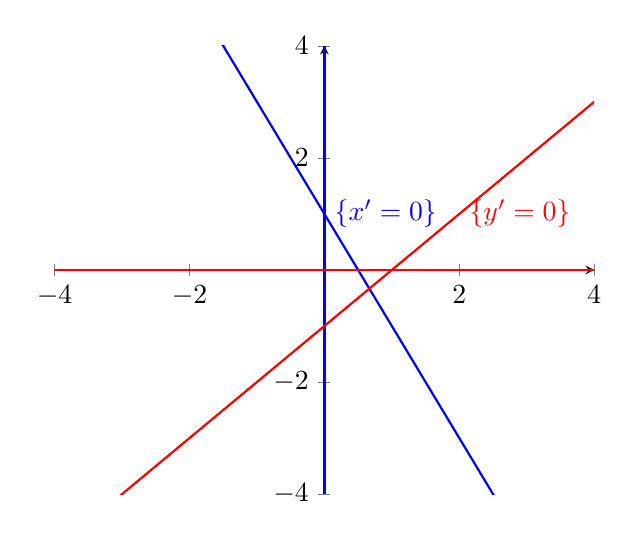
\begin{tikzpicture}
				\begin{axis}[ymin=-4,
						ymax=4,
						xmin=-4,
						xmax=4,
						samples=50,
						axis y line=middle,
						axis x line=middle]
					\addplot[thick,blue] {1 - 2 * x} node[pos=0.5,right] {$\{ x' = 0 \}$};
					\addplot[thick,blue] coordinates {(0,-4)(0,4)};
					\addplot[thick,red] {x - 1} node[pos=0.7,right] {$\{ y' = 0 \}$};
					\addplot[thick,red] {0};
				\end{axis}
			\end{tikzpicture}
		\end{center}
	\end{otherlanguage}
	נעבור לחישוב הקבוצה ברביע הראשון שבה $x' > 0$, כמסקנה מהחישוב הקודם נקבל $\{ x, y \ge 0 \mid y < 1 - 2x \}$ ולכן גם $\{ x' < 0 \} = \{ 1 - 2x < y \}$ ונשרטט,
	\begin{otherlanguage}{english}
		\begin{center}
			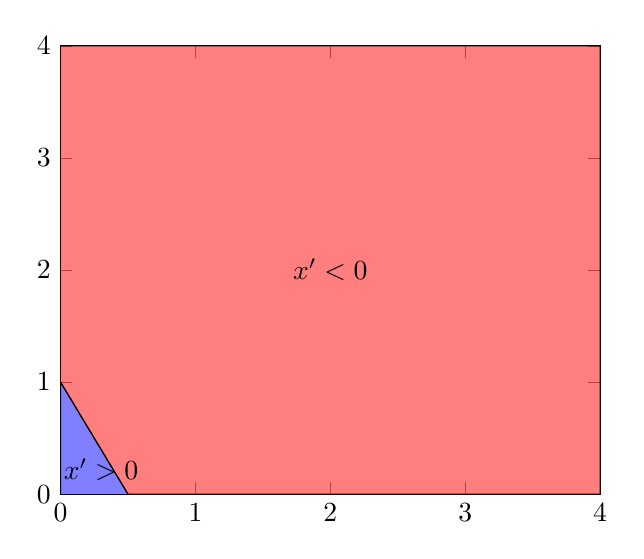
\begin{tikzpicture}
				\begin{axis}[ymin=0,
					ymax=4,
					xmin=0,
					xmax=4,
					samples=50]
					\addplot[fill=blue, fill opacity=0.5] coordinates {
						(0,0)
						(0,1)
						(0.5,0)
					};
					\addplot[fill=red, fill opacity=0.5] coordinates {
						(0,1)
						(0.5,0)
						(4,0)
						(4,4)
						(0,4)
					};
					\node at (axis cs:0.3,0.22) {$x' > 0$};
					\node at (axis cs:2,2) {$x' < 0$};
				\end{axis}
			\end{tikzpicture}
		\end{center}
	\end{otherlanguage}
	ושוב באותו חישוב נקבל,
	\begin{otherlanguage}{english}
		\begin{center}
			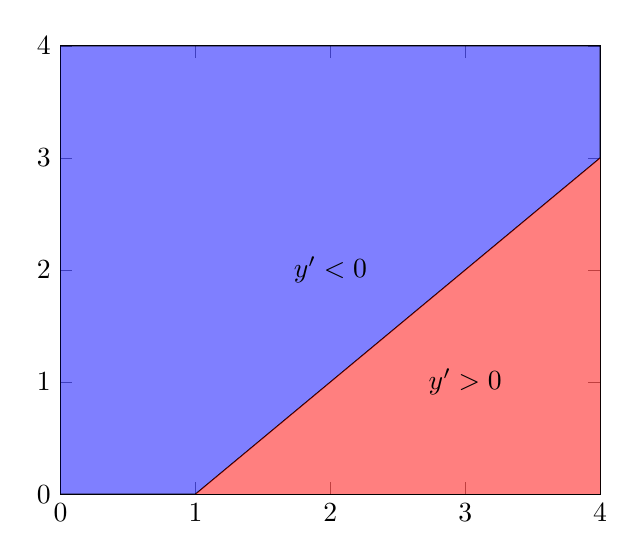
\begin{tikzpicture}
				\begin{axis}[ymin=0,
					ymax=4,
					xmin=0,
					xmax=4,
					samples=50]
					\addplot[fill=blue, fill opacity=0.5] coordinates {
						(0,0)
						(1,0)
						(4,3)
						(4,4)
						(0,4)
					};
					\addplot[fill=red, fill opacity=0.5] coordinates {
						(1,0)
						(4,0)
						(4,3)
					};
					\node at (axis cs:2,2) {$y' < 0$};
					\node at (axis cs:3,1) {$y' > 0$};
				\end{axis}
			\end{tikzpicture}
		\end{center}
	\end{otherlanguage}
\end{solution}

\subquestion{}
נראה כי כל הפתרונות שמתחילים ברביע הראשון מתכנסים לנקודת שיווי משקל כלשהי של המערכת.
\begin{proof}
	בתחום זה יש רק שתי נקודות שיווי־משקל והן $(0, 0), (\frac{1}{2}, 0)$, נראה שכל פתרון שמתחיל ברביע הראשון מתכנס לאחת מהן.
	בהשראת השרטוטים נספק הוכחה גאומטרית ולא הוכחה פורמלית.
	לכל נקודה בה $y' > 0$ מתקיים $x' < 0$ ולכן תמיד היא תגיע לסביבה בה $y' < 0$, באופן דומה לכל נקודה בה $x' < 0$ נקבל הגעה לנקודה $(\frac{1}{2}, 0)$ או עלייה וירידה סביבה $(1,1), (\frac{1}{2},0)$.
	בסביבה זו $y \to 0$ ולכן נקבל את המבוקש.
\end{proof}

\question{}
יהי $F : \Omega \to \RR^n$ שדה גזיר ברציפות כך ש־$0$ נקודת שיווי־משקל של המערכת $x' = F(x)$.
נסמן $A = D_0 F$ ונניח שכל הערכים העצמיים של $A$ בעלי חלק ממשי שלילי.

\subquestion{}
נראה כי האינטגרל,
\[
	S
	= \int_{0}^{\infty} {\exp(t A)}^t \exp(t A)\ dt
\]
קיים וסופי וכן ש־$S$ מטריצה חיובית בהחלט ושלכל $x \in \RR^n$ מתקיים,
\[
	\langle S x, A x \rangle
	= -\frac{1}{2} \lVert x \rVert_2^2
\]
\begin{proof}
	יהי $\max_{\lambda \in \Lambda} \re \lambda < \alpha < 0$ כאשר $\Lambda$ קבוצת הערכים העצמיים של $A$.
	בכיתה הוכחנו שקים $C > 0$ כך שמתקיים,
	\[
		\forall t \ge 0,
		\quad
		\lVert e^{t A} \rVert_{op}
		< C e^{t \alpha}
	\]
	מאי־שוויון המשולש ואי־שוויון זה נקבל,
	\begin{align*}
		\left\lVert \int_{0}^{\infty} {\exp(t A)}^t \exp(t A)\ dt \right\rVert_{op}
		& \le \int_{0}^{\infty} \lVert {\exp(t A)}^t \rVert_{op} \cdot \lVert \exp(t A) \rVert_{op}\ dt \\
		& \le \int_{0}^{\infty} C e^{t \alpha} \cdot C e^{t \alpha}\ dt \\
		& = C^2 \int_{0}^{\infty} e^{t 2\alpha}\ dt \\
		& = C^2 \cdot \frac{1}{2 \alpha} (1 - 0)
	\end{align*}
	ובפרט האינטגרל מתכנס בהחלט (עד כדי משפט שקילות הנורמות) ולכן $S$ מוגדר וסופי.
	
	ישירות מלינארית והעובדה ש־$A$ ממשית נסיק ש־${\exp(t A)}^t \exp(t A)$ היא חיובית לחלוטין, ומתכונות אינטגרל על מטריצה כאינטגרל איבר איבר נקבל שגם $S$ מטריצה חיובית לחלוטין וסימטרית.

	עתה נבחין כי גם,
	\[
		\int_{0}^{\infty} \frac{d}{dt} ({\exp(t A)}^t \exp(t A))\ dt
		= 0 - I
	\]
	מהרחבה של המשפט היסודי של החשבון האינפיניטסימלי.
	מהצד השני,
	\[
		\frac{d}{dt} ({\exp(t A)}^t \exp(t A))\ dt
		= A {\exp(t A)}^t \exp(t A) + A^t {\exp(t A)}^t \exp(t A)
	\]
	ולכן,
	\[
		\int_{0}^{\infty} \frac{d}{dt} ({\exp(t A)}^t \exp(t A))\ dt
		= A S + S A^t
	\]
	לכן,
	\[
		-I = A S + S A^t
	\]
	בנוסף נבחין כי $x^t A S x = {(x^t S^t A^t x)}^t = x^t S A^t x$ מסימטריה של $S$ והעובדה שזהו כפל פנימי ולכן סקלר (וסימטרי), אז גם,
	\[
		\langle S x, A x \rangle
		= x^t S A x
		= \frac{1}{2} x^t A S x + \frac{1}{2} x^t S A^t x
		= \frac{1}{2} x^t (A S + S A^t) x
		= \frac{1}{2} x^t (-I) x
		= -\frac{1}{2} \lVert x \rVert_2^2
	\]
	וקיבלנו את התוצאה המבוקשת.
\end{proof}

\subquestion{}
נראה כי $L(x) = \langle S x, x \rangle$ היא פונקציית ליאפונוב חזקה של $F$ בסביבה של $0$,
ונסיק כי $0$ נקודת שיווי משקל אסימפטוטית של המערכת $F$.
\begin{proof}
	נראה ש־$\langle \nabla L(x), F(x) \rangle < 0$ לכל $x \ne 0$.
	\[
		\nabla L(x)
		= (\langle \frac{d}{d x_1} S x, x \rangle + \langle S x, e_1 \rangle, \ldots, \langle \frac{d}{d x_n} S x, x \rangle + \langle S x, e_n \rangle)
		= 2 S x
	\]
	ובסביבה מספיק קטנה של $0$ מתקיים,
	\[
		F(x)
		= F(0) + A x + o(\lVert x \rVert_2)
		= A x + o(\lVert x \rVert_2)
	\]
	ואם נציב נקבל,
	\[
		\langle \nabla L(x), F(x) \rangle
		= \langle 2S x, A x + o(\lVert x \rVert) \rangle
		= \langle 2S x, A x \rangle + \langle 2S x, o(\lVert x \rVert) \rangle
		= 2 \cdot (-\frac{1}{2}) \lVert x \rVert_2^2 + \varepsilon
		= - \lVert x \rVert_2^2 + \varepsilon
		< 0
	\]
	כאשר $\varepsilon > 0$ קטן כרצננו ביחס ל־$\lVert x \rVert$ על־ידי בחירת הסביבה. \\
	נבחין כי $L(x) = x^t S x$ עבור פונקציה סימטרית וחיובית לחלוטין ולכן מלינארית $L(x) \ge 0$ וכן $L(x) = 0 \iff x = 0$ וקיבלנו ש־$L$ ליאפונוב על־פי ההגדרה.

	ממשפט ליאפונוב נסיק ש־$0$ נקודת שיווי משקל יציבה אסימפטוטית של $x' = F(x)$.
\end{proof}

\end{document}
